This is the first interface that is shown to the user. This is the Home page.
It brings a nice UI to get input from user about the Number of storeys and 
some factor affecting the structure. It also provides the user some 
additional features as an aid like uploading data as CSV files and Email 
after completion. There is an additional help icon near every field to get 
an idea of what it is. There is a static navigation bar that provides an 
Autofill values option. By clicking that option, default values are 
automatically filled.

\begin{figure} 
\centering 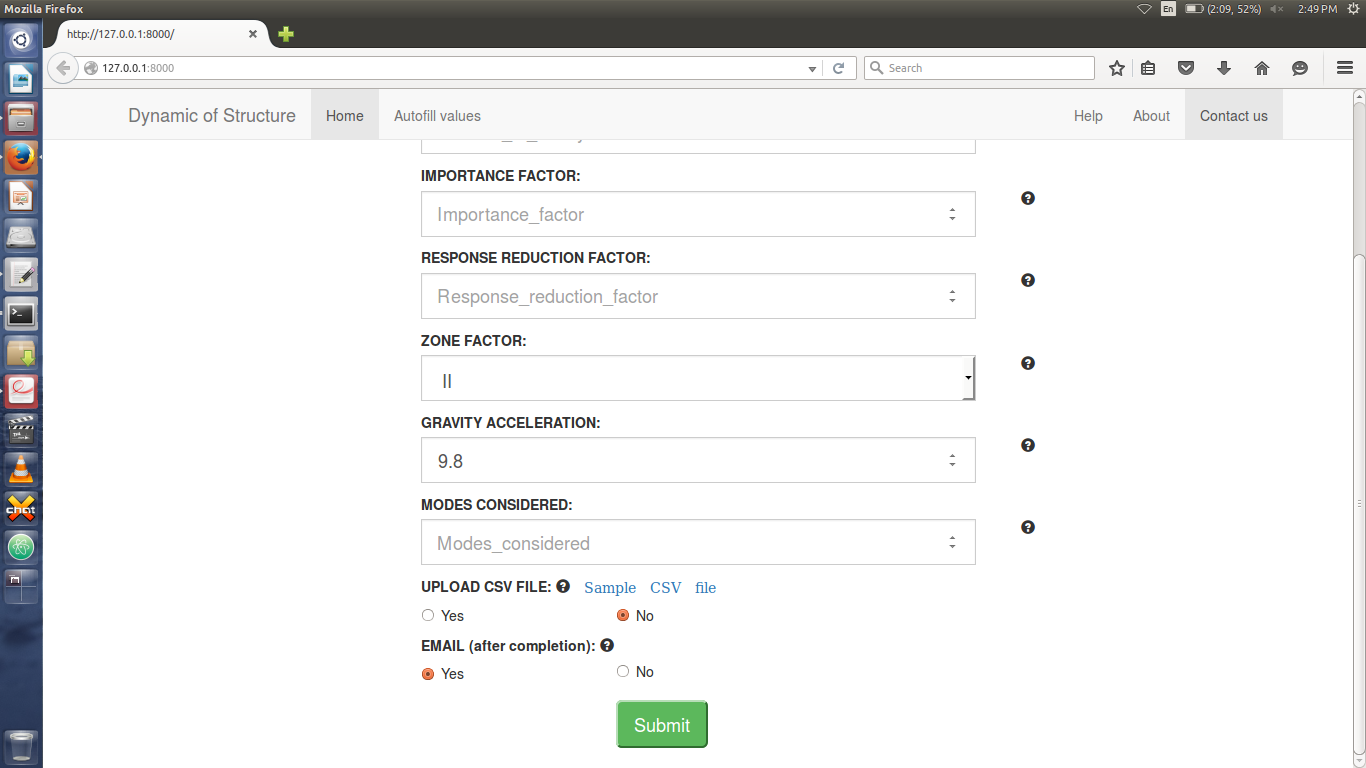
\includegraphics[scale=0.32]{images/output/1.png}
\caption{Home page of DoS}
\end{figure}

After clicking the 'Submit' button on the homepage, user is shown another 
form based on his input "Number of Storeys" in the homepage form, for 
filling out the matrix values manually.

\begin{figure} 
\centering 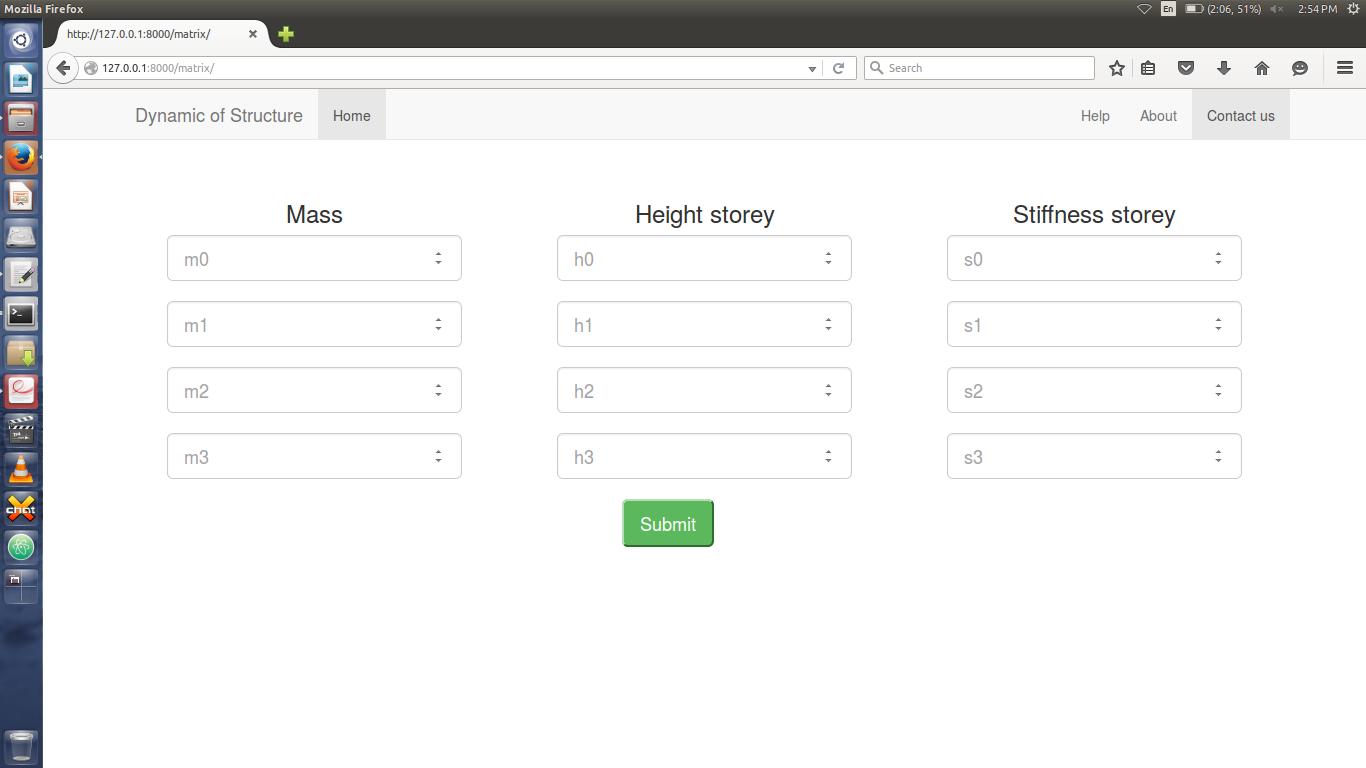
\includegraphics[scale=0.32]{images/output/2.png}
\caption{Matrix.html for manually filling values}
\end{figure}

The top navigation bar is static to all pages. There is a link to the Help. 
After clicking which, the help regarding the different inputs fields 
provided.

\begin{figure} 
\centering 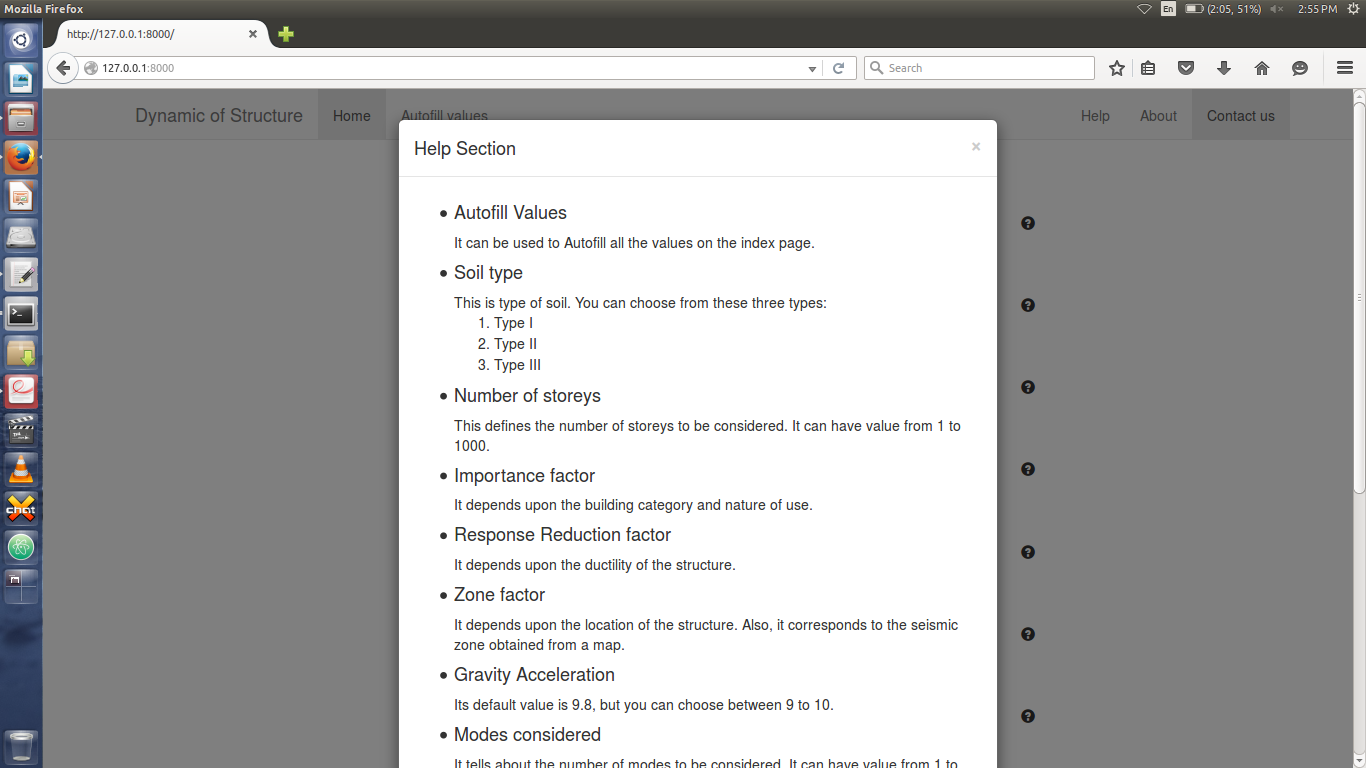
\includegraphics[scale=0.31]{images/output/3.png}
\caption{Help section in Home page}
\end{figure}

There are small icons near each of the input field on the homepage. They are 
the help icons. After hovering them, they display a little help related to
that correspond field.
\begin{figure} 
\centering 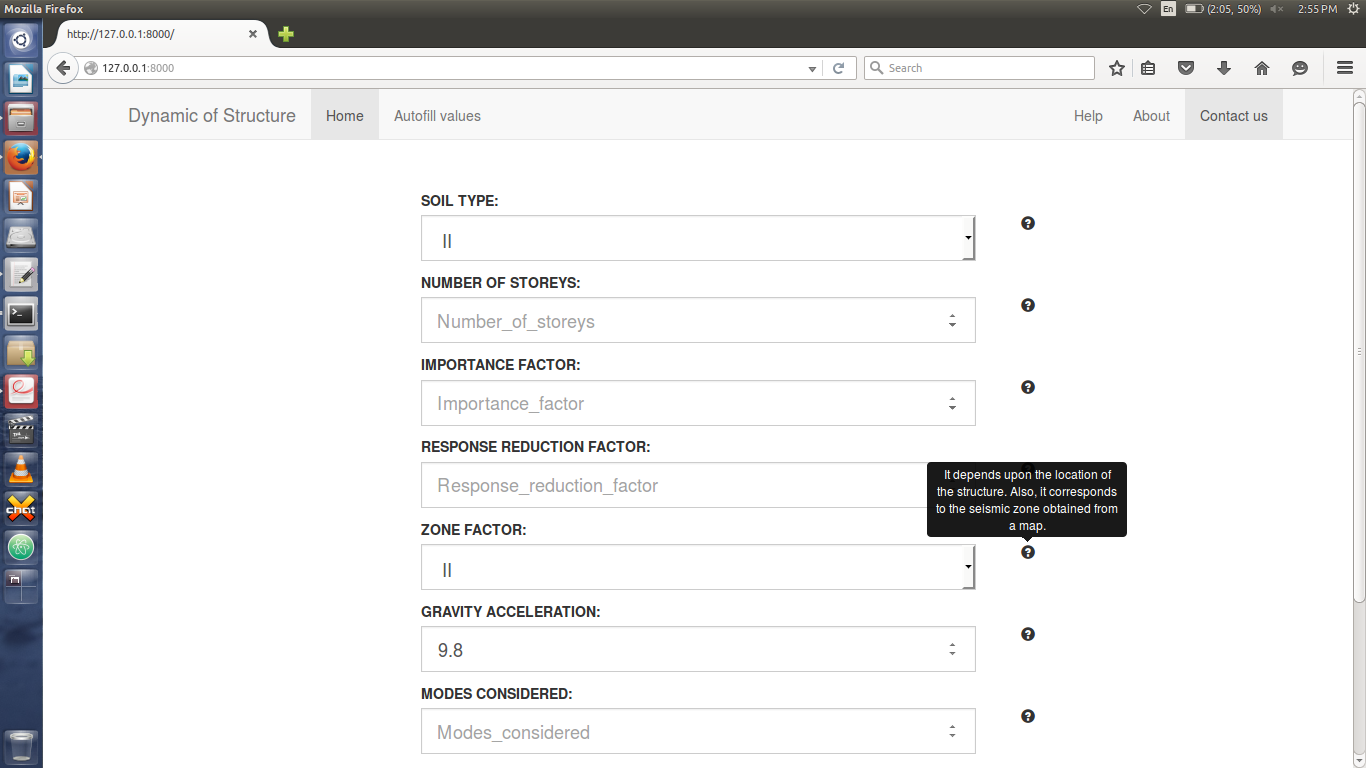
\includegraphics[scale=0.31]{images/output/4.png}
\caption{Local help option}
\end{figure}

After running a set of commands of \LaTeX and SageMath, it produces the
output in PDF form (with pdflatex).
\begin{figure} 
\centering 
\includegraphics[scale=0.31]{images/output/6.png}
\caption{First page of PDF generated by DoS}
\end{figure}

After the titlepage, table of content and some other stuff, the PDF contains 
the values (matrices) entered in the form at the homepage.
\begin{figure} 
\centering 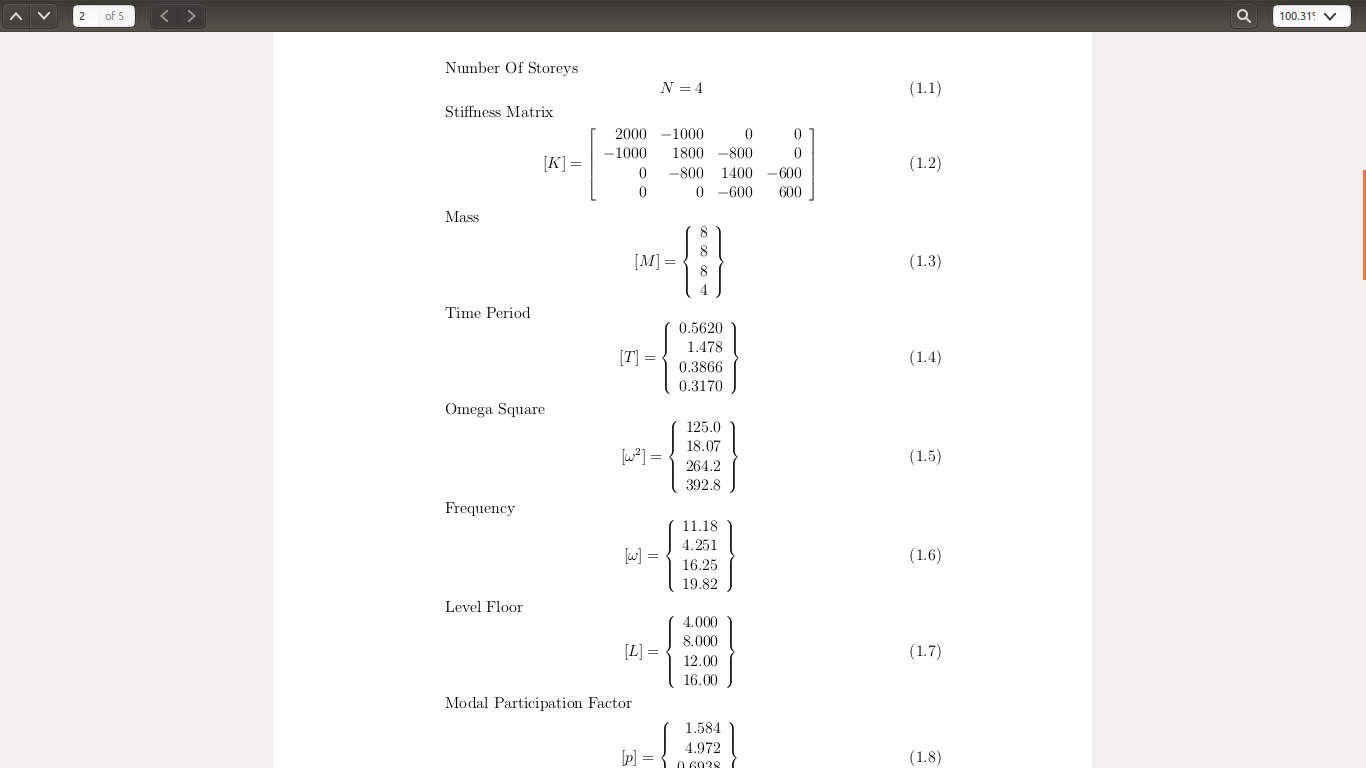
\includegraphics[scale=0.31]{images/output/7.png}
\caption{Initial values given for checking in PDF}
\end{figure}

There is graph embedded in the PDF which is being created using Sagemath.
\begin{figure} 
\centering 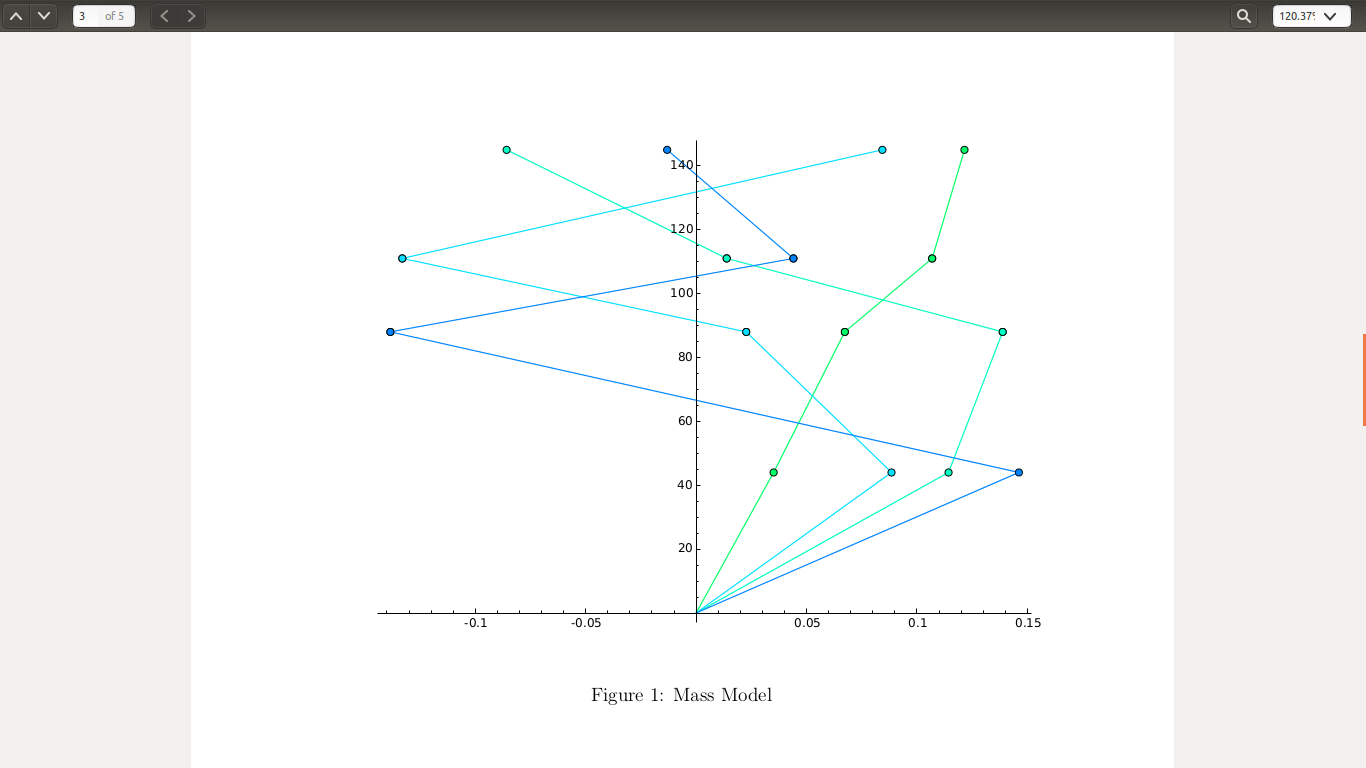
\includegraphics[scale=0.31]{images/output/8.png}
\caption{Graph Generated in PDF}
\end{figure}

After all calculations, the computed final result is printed on the PDF.
\begin{figure} 
\centering 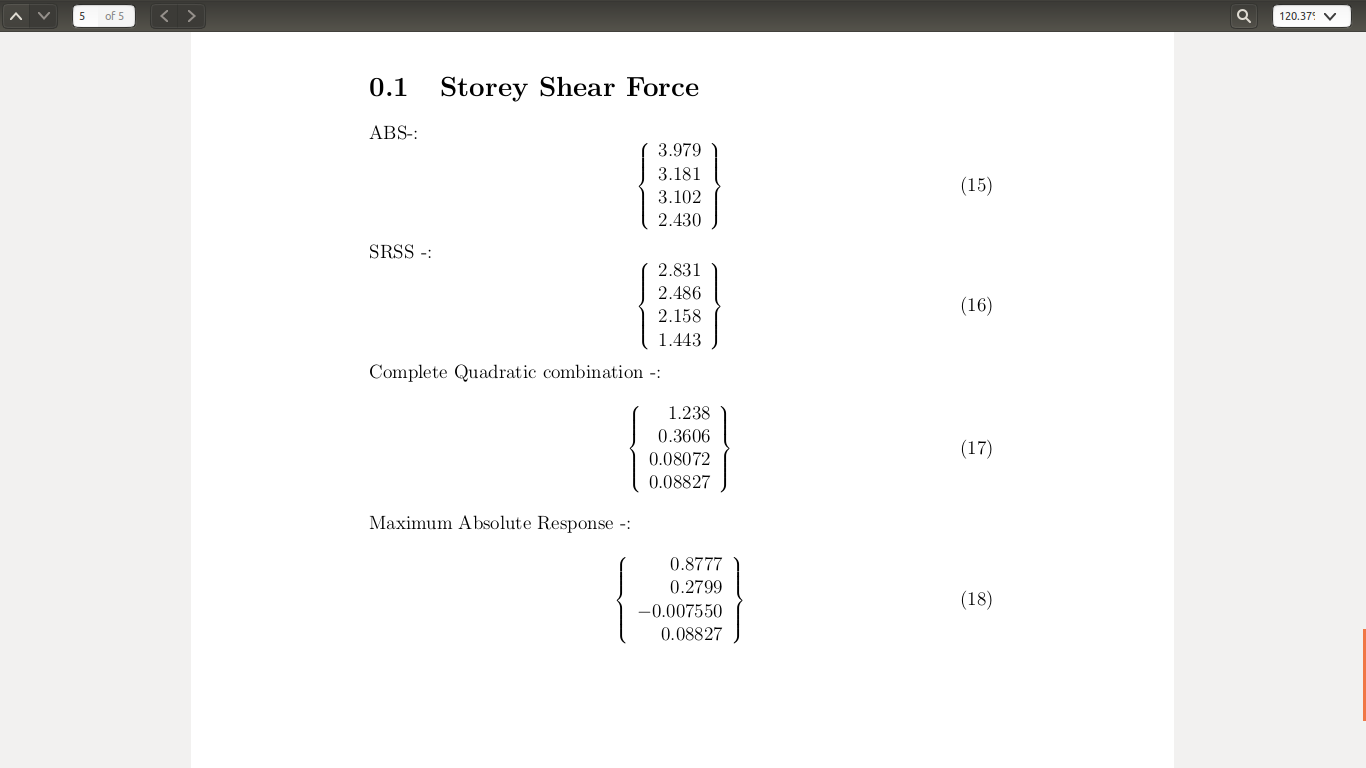
\includegraphics[scale=0.31]{images/output/9.png}
\caption{Final output in PDF}
\end{figure}
